\documentclass[10 pt, twocolumn]{article}

\usepackage[utf8]{inputenc}
\usepackage[T1]{fontenc}
\usepackage{caption}
\usepackage{graphicx}
\usepackage{xcolor}
\usepackage{interval}
\usepackage{listingsutf8}
\usepackage{hyperref}
\usepackage{siunitx}
\usepackage{algorithm2e}
\usepackage{rotating}
\usepackage{adjustbox}
\usepackage{booktabs}
\usepackage{pgfplots}
\usepackage{tikz}
\usepackage{footmisc}
\usepackage{amsfonts}
\usepackage[backend=biber,style=numeric]{biblatex}
\usepackage[
  left=1.50cm,
  right=1.50cm,
  top=2.00cm,
  bottom=2.00cm
]{geometry}

\pgfplotsset{compat=1.15}

\sisetup{load-configurations=abbreviations, binary-units=true}
\intervalconfig {
    soft open fences ,
    separator symbol =; ,
}

\lstdefinelanguage{JavaScript}{
  keywords={break, case, catch, continue, debugger, default, delete, do, else, finally, for, function, if, in, instanceof, new, return, switch, this, throw, try, typeof, var, void, while, with},
  morecomment=[l]{//},
  morecomment=[s]{/*}{*/},
  morestring=[b]',
  morestring=[b]",
  sensitive=true
}

\lstdefinelanguage{Protobuf}{
  keywords={message, string, uint32, int32},
  morecomment=[l]{//},
  morecomment=[s]{/*}{*/},
  morestring=[b]',
  morestring=[b]",
  sensitive=true
}

\lstset{
    language=C,
    keywordstyle={\bfseries},
    basicstyle=\footnotesize,
    literate={->}{$\rightarrow{}$}{1} {<-}{$\leftarrow{}$}{1},
    stringstyle=\color{purple},
    keepspaces=true,
    captionpos=b,
    inputencoding=utf8,
    escapeinside={\%*}{*)}
}

\renewcommand\AlCapSty{\text}
\SetAlCapNameFnt{\footnotesize}
\SetAlCapFnt{\footnotesize}
\SetAlgoCaptionSeparator{.}
\DeclareCaptionLabelFormat{nospace}{#1 #2}
\captionsetup[table]{labelformat=nospace,labelfont=rm,name=Table,labelsep=period}

\newcommand{\pcode}[1]{
    \lstinline[basicstyle=\itshape,keywordstyle={}]{#1}
}

\newcommand*{\lstnumberautorefname}{line}

\newcommand{\icode}[1]{\lstinline{#1}}

\newcommand{\name}[1] {\emph{#1}}

\newcolumntype{R}[2]{%
    >{\adjustbox{angle=#1,lap=\width-(#2/2)}\bgroup}%
    l%
    <{\egroup}%
}
\newcommand*\rot{\multicolumn{1}{R{90}{1em}}}

\newcommand{\fig}[3]{
  \begin{figure}[h]
    \begin{center}
        \includegraphics[width=8cm,keepaspectratio]{#1}
        \caption{#3}
        \label{fig:#2}
    \end{center}
  \end{figure}
}

\usepackage[most]{tcolorbox}
\newcounter{example}
\usepackage{xparse}
\usepackage{lipsum}

\def\exampletext{Example} % If English
\NewDocumentEnvironment{example}{ O{} }
{
\colorlet{colexam}{red!55!black} % Global example color
\newtcolorbox[use counter=example]{examplebox}{%
    % Example Frame Start
    empty,% Empty previously set parameters
    title={#1},% use \thetcbcounter to access the example counter text
    % Attaching a box requires an overlay
    attach boxed title to top left,
       % Ensures proper line breaking in longer titles
       minipage boxed title,
    % (boxed title style requires an overlay)
    boxed title style={empty,size=minimal,toprule=0pt,top=4pt,left=3mm,overlay={}},
    coltitle=colexam,fonttitle=\bfseries,
    before=\par\medskip\noindent,parbox=false,boxsep=0pt,left=3mm,right=0mm,top=2pt,breakable,pad at break=0mm,
       before upper=\csname @totalleftmargin\endcsname0pt, % Use instead of parbox=true. This ensures parskip is inherited by box.
    % Handles box when it exists on one page only
    overlay unbroken={\draw[colexam,line width=.5pt] ([xshift=-0pt]title.north west) -- ([xshift=-0pt]frame.south west); },
    % Handles multipage box: first page
    overlay first={\draw[colexam,line width=.5pt] ([xshift=-0pt]title.north west) -- ([xshift=-0pt]frame.south west); },
    % Handles multipage box: middle page
    overlay middle={\draw[colexam,line width=.5pt] ([xshift=-0pt]frame.north west) -- ([xshift=-0pt]frame.south west); },
    % Handles multipage box: last page
    overlay last={\draw[colexam,line width=.5pt] ([xshift=-0pt]frame.north west) -- ([xshift=-0pt]frame.south west); },%
    }
\begin{examplebox}}
{\end{examplebox}\endlist}

\newcommand*\circled[1]{\tikz[baseline=(char.base)]{
            \node[shape=circle,draw,inner sep=1pt] (char) {#1};}}

\usepackage{tikz}

\newcommand{\smiley}{\tikz[baseline=-0.75ex,black]{
    \draw circle (2mm);
\node[fill,circle,inner sep=0.5pt] (left eye) at (135:0.8mm) {};
\node[fill,circle,inner sep=0.5pt] (right eye) at (45:0.8mm) {};
\draw (-145:0.9mm) arc (-120:-60:1.5mm);
    }
}

\newcommand{\frownie}{\tikz[baseline=-0.75ex,black]{
    \draw circle (2mm);
\node[fill,circle,inner sep=0.5pt] (left eye) at (135:0.8mm) {};
\node[fill,circle,inner sep=0.5pt] (right eye) at (45:0.8mm) {};
\draw (-145:0.9mm) arc (120:60:1.5mm);
    }
}

\newcommand{\neutranie}{\tikz[baseline=-0.75ex,black]{
    \draw circle (2mm);
\node[fill,circle,inner sep=0.5pt] (left eye) at (135:0.8mm) {};
\node[fill,circle,inner sep=0.5pt] (right eye) at (45:0.8mm) {};
\draw (-135:0.9mm) -- (-45:0.9mm);
    }
}


\addbibresource{root.bib}

\title{So you want to build a ML system}

\author{Jan Macháček}

\begin{document}

\twocolumn[
  \begin{@twocolumnfalse}
    \maketitle
    \begin{abstract}
      Amongst other things, a machine learning system should be built! It can solve anything, there are so many wonderful frameworks, so many conference talks that show just how easy it is to throw together just a few line of Python, and hey presto!--a machine that can recognise digits in images, recognise hot dog and \emph{not} hot dog... it even runs on a mobile phone. This essay is about the difficulties that are lurking in the execution and running of a robust \& mature machine learning system.
    \end{abstract}
  \end{@twocolumnfalse}
]

\section{What can ML do?}
The exercise analysis system sets out to be a computerized personal for resistance or strength exercise. Exercise systems collect heart rate data as the baseline indication of physical exertion. Depending on the chosen sport, the systems typically collect GPS and accelerometer data. Geo-location, acceleration, and heart rate are fairly comprehensive source of data for outdoors sports: think running or cycling. For cycling, geo-location sampled at, say, \SI{50}{\hertz} reliably establishes the route ridden, but is also the source of data for speed and acceleration; with underlying elevation data \& the weight of the rider and the bicycle, it is possible to estimate power output. With the heart rate, it is possible to get a  fairly accurate view of the activity in \autoref{fig:cycling-overall}.

\fig{cycling-overall.png}{cycling-overall}{An afternoon ride}

In addition to the post-ride analysis, the sensors provide immediate feedback during the ride. A modern cycling computer records and displays speed, elevation, distance, heart rate, pedalling cadence, and power. An athlete can use these values to inform his or her training; for example, one might train for a time trial aiming for a particular power output over a specific distance and use the values a cycling computer displays to guide the training sessions. (See \autoref{fig:cycling-power-training}.)

\fig{cycling-power-training.jpg}{cycling-power-training}{Cycling power training}

Everything becomes much more difficult indoors; and then even more difficult when not in a swimming pool, on a rowing machine, or on a spinning bike; when the user turns to resistance exercise. Some exercise machines now come with Bluetooth ``beacons'' that advertise the details of the activity. Any sensors are less likely to be embedded in free weights (and even if there were sensors, the sensors cannot reveal the exercise the user is performing; though identification such as \SI{20}{\kg} dumbbell is useful, and acceleration \& rotation is even more useful). There are no machines involved at all in body-weight exercises. 

To build a system for resistance exercise analysis that ``matches'' the features of a cycling system \emph{without requiring super high-tech gym}, it will be necessary for the users to \emph{bring their own sensors}. A smart-watch can provide acceleration, rotation, and heart rate\footnote{Though most smart-watches report ``beats per minute'', the watch measures changes of the blood flow velocity, which is directly correlated to heart rate. Nevertheless, the watch does not measure heart rate itself.}; these three sensor readings can be fused with sensor readings from a smart-phone that the user might wear in his or her pocket. This gives additional acceleration and rotation. Unfortunately, heart rate lags behind any exertion, so it'll only increase by the time the user is done with a set of a particular exercise (assuming the exercise is done with appropriate intensity); the last easily accessible sensor, geo-location (if at all available due to the location of the exercise floor) will show that the user is not moving much. This leaves only the acceleration and rotation values as useful indications of the movement being performed. 

A proof-of-concept application that allows the users to wear a sensor on their wrists and use their mobile phones to \emph{mark the start and end of each exercise}, together with \emph{the name of the exercise} provides the data to build \& verify the first models. 

\fig{exercise-a.png}{exercise-a}{Two exercises}

\autoref{fig:exercise-a} shows the acceleration from a watch worn on the left wrist. The acceleration is along the $x$, $y$, and $z$ axes (with the Earth contributing \SI{9.8}{\meter\second^{-2}}) sampled at \SI{50}{\hertz}; exercise \circled{1} is the straight bar biceps curl, and \circled{2} is the chest dumbbell flyes. You--the readers, humans--can work out the number of repetitions and you can clearly spot that these are two different exercises, and if you saw enough of these figures, you would be able to learn to identify the two exercises. It should be possible to implement a function \pcode{classify(sensor data) -> exercise} that does the same. Even if this function performs perfectly (i.e. it identifies the movement that corresponds to the exercise for every \pcode{sensor data} that matches the exercise, even if the exact \pcode{sensor data} was not in the training set), it will struggle to identify areas of no exercise; unfortunately no exercise does not mean no movement, it simply means that the user is walking from one machine to another, setting up for a different exercise, taking a drink, and so on. These no exercise areas are quite often also areas of repetitive motion (walking) or fairly large movements (setting up); see \autoref{fig:exercise-vs-slacking} where the red shaded areas represent exercise and the rest is other recorded motion.

\fig{exercise-vs-slacking.png}{exercise-vs-slacking}{Exercise vs. slacking}

The figure shows some of the typical challenges of noisy and mislabelled data. For example in \circled{1}, the user has done two exercise sets, but forgot to label the no exercise area properly. The area in \circled{2} shows large movement in the no exercise section--in this particular example, the acceleration actually shows the user dragging an exercise bench. In \circled{3}, the labelling is not entirely accurate: the user started the label before actually starting the exercise. Finally, \circled{4} shows further wide movements in the no exercise section. To deal with the complexity of exercise and no exercise, the classification function needs to be \pcode{classify(sensor data) -> result}, where \pcode{result = exercise | no-exercise}. 

\subsection{Sensors are not enough}
Suppose there is indeed a function\cite{Knight:2006ki}, \cite{Morris:2014ir} that takes the sensor readings and returns the details of the exercise being performed: \pcode{classify(sensor data) -> result}. Even if this function performs perfectly, it only allows to build a system that lags behind the users' movement. Even if the system could read the data from the sensors with zero delay, the system would only be able to tell the user what he or she is doing after ``seeing'' some minimum amount of data, introducing lag. High lag will cause the user experience to be rather frustrating. In our testing, a \SI{100}{\milli\second} lag is noticeable; \SI{250}{\milli\second} lag is still tolerable; anything over \SI{750}{\milli\second} is downright confusing. A good example is the number of repetitions: with an exercise whose single repetition takes around \SI{1}{\second}, a \SI{750}{\milli\second} lag will mean that the system shows 5\textsuperscript{th} repetition when in fact the user is starting on his or her 7\textsuperscript{th}. Compare this to the sensor readings that the cycling computer reports: speed, altitude and similar can be reported as they are measured (typically a few times per second); cadence and power readings usually lag behind the instantaneous measurements because the computers display average values over a short time window. Just like the repetitions in resistance exercise, the lag is confusing; though if the athlete holds fairly steady power output, the reading usually matches the perceived effort.

The machine learning resistance exercise system is competing with a simple exercise log on paper notebook. Following users that use such an \emph{ancient} technology reveals the flow that the application has to satisfy. 

\fig{diary.jpg}{diary}{Exercise diary}

The athletes use a diary similar to the one in \autoref{fig:diary} to log the exercises done, to keep track of progress, and to stick to an established sequence of exercises. The interaction the users need is for the application to show \emph{what to do next}, with all relevant details of weights, repetitions, time, and intensity. This is what a user would be able to trivially look up in the paper diary. The paper diary also easily deals with the scenario when there the exercise space or machine is not available: it is trivial to scan the diary for the alternative exercise. So, the mobile application's interactions need to match that. (See \autoref{fig:ui}.)

\fig{ui.jpg}{ui}{Electronic version of exercise diary}

The model used to predict sequence of exercise sessions and exercises within a session is a Markov chain. This allows the application to deal with the reality of exercise in a public gym, where the station for the next suggested exercise might not be available. The Markov chain, together with a bio-mechanical model of the main muscle groups, gives the users the flexibility to achieve their workout targets even in crowded gyms. The sequence of exercise predictions for one particular exercise sessions are illustrated on \autoref{fig:model-sequence}.

\fig{model-sequence.png}{model-sequence}{Exercise sequence model with no context}

The numbers in \autoref{fig:model-sequence} represent the count of transitions taken; hence it is possible to calculate the probability of transition from any given state. The state names are the exercise labels, in real application, they are the real exercise names. The mobile application can either receive the chain when the user selects one of the pre-defined exercise programmes, or it can construct the chain from empty if the user chooses to start his or her custom workout. This gives the application an intuitive feel; its suggestions are what the users usually do. Finally, the information in the chain allows the system to identify the most popular sequences of exercises, to identify exercises that the users do not like; more interestingly, the system can use the information in the chain to identify sequence of exercises that leads to the best improvement. (There is no definition of \emph{improvement}: in one case, it may be greatest perceived intensity; in other case, it may be greatest mobility range improvement; etc.)

To make the next-exercise prediction more accurate, the mobile application uses fined-grained location services. The location services are implemented using bluetooth beacons. The beacons operate in the iBeacon mode \cite{ibeacon}; each beacon in this mode transmits its identifier, a major, and minor values. The mobile application sets up continuous scanning of a major value which identifies exercise equipment, receiving notifications of beacons and their minor values as they come into range. The mobile application then filters the exercise states keeping only those that are associated with a particular area.

With the fine-grained location data available, the application is \emph{expecting} to see a movement that precedes exercises A or C. We call this movement the \emph{set-up movement}. This now refines the classification into the \name{setup movement} classifier and the \name{in-exercise} classifier. Both classifiers follow the general \pcode{classify(sensor data) -> result} signature. The set-up movement classifier takes \SI{1}{\second} of sensor input and produces probabilities classes that represent the set-up movement for groups of exercises. The set-up classes are not the exercises themselves, but the movements that happen just before the start of an exercise (think picking up the dumbbells and moving them into place for shoulder press); one set-up movement can map to multiple exercises. To provide accurate prediction of the exercise about to be started, the mobile application takes into account the expected exercise (given the user's typical behaviour), and the fine-grained location data. \autoref{fig:pc-chain} illustrates the sequence of predictors and classifiers.

\fig{pc-chain.png}{pc-chain}{Predictors and classifiers}

Note that the predictors' outputs change over time: at time $0$ the probability of \emph{rest} is $0.8$, and the probability of any exercise is $0$; as time increases towards $1$, the probability of \emph{rest} decreases, and the probability of exercises ${A, B, C}$ increases, especially when taking into account that the fine-grained location sensor reports being in proximity of the weights rack. In the time interval $\interval[open]{1}{2}$, the probability of exercises ${A, B, C}$ steadily decreases, and the probability of \emph{rest} increases. If (particularly at the start) of the time interval $\interval[open]{1}{2}$, the \name{set-up classifier} classifies movement that is consistent with the set-up movement for muscle groups ${\alpha, \omega}$ (where $\alpha$ contains exercises ${A, C, ...}$ and $\omega$ contains exercises ${B, X, ...}$), the system can deduce that the user is likely to be getting ready to perform exercise $A$ or $C$. The details of the likely exercises are passed to the \name{in-exercise signal processor}, which is responsible for counting repetitions and evaluating the variation in the acceleration that is indicative of effort. The same information (set-up movement ${\alpha, \omega}$, expected exercises ${A, C, B}$) is fed to the \name{in-exercise} classifier, which seeks to confirm that the exercise being done is indeed $A$. In gym-speak, the muscle group $\alpha$ can be \name{shoulders} and $\omega$ can be \name{upper back}; the exercise $A$ can be \name{dumbbell shoulder press}, and $C$ \name{barbell shoulder press}. The final task for the application is to associate effort (measured by the \name{in-exercise signal processor}) with weight. It uses a map of \pcode{(exercise, sequence number, effort) -> weight} that it maintains for each user. (It is important to keep track of the \pcode{sequence number}, especially for high-intensity work.)

The performance of the entire prediction and classification flow exercise prediction for accelerometer and gyroscope on the user's wrist and accelerometer and gyroscope in the user's mobile in the left pocket is shown in TODO: Chart here.

\section{Bootstrapping}
I knew what I was getting into when I was building the application and when I was using it in the gym. It was clear that at the start, there are no transitions from one exercise to another, no maps of \pcode{effort -> weight}, that the classifiers and signal processors' parameters are not tuned or trained. Using the application's labelling interface and the old-school diary, it was possible to collect enough data for all components to perform as well as the tables above show. 

The data used to train the \name{set-up movement} and \name{in-exercise} classifiers is re-usable\footnote{The test users' athletic abilities were similar to the author's}, and a lot of training data can be generated by using the raw readings as inputs to a bio-mechanical model, which then generate the actual training and validation data for the classifiers. However, the exercise sequences in the Markov chains have proven to be very different between the users. The application required utmost patience during the first several exercise sessions. This was acceptable in the friendly test group, but would turn out to be a significant problem for a commercial application. An acceptable solution--from the user experience as well as accuracy point--is to run the application in \emph{observer} mode for the first 10 sessions. In the observer mode, it does not suggest or classify anything; it submits the recorded data to the server-side for deeper classification. The server-side classifiers reconstruct the exercise sequences and then provide the parameters for the predictors. After the initial observer mode, the users\footnote{Embarrassingly, $N=10$.} report that the application ``does the right thing.''

\section{The complexity of sensors}
The system reads values from the sensors; the values are not read continuously, but read at discrete points in time. The range of sensor values can introduce clipping errors, and the sampling rate can introduce aliasing errors. Good choice of sampling rate and sensor types can reduce these errors: both sampling rates and sensor value range must be significantly greater than expected measurements; even in that case, the system must include enough signal processing to eliminate rogue values. For humans in resistance exercise, the sampling rate is sufficient to be \SI{50}{\hertz}, acceleration is expected to be in the range \SI{\pm40}{\meter\second^{-2}}, rotation \SI{\pm4\pi}{\radian\second^{-1}}. The first stab at implementing the sensor reading code may take the form of a loop in \autoref{alg:naive-sensor-sampling}.

\begin{algorithm}
  \caption{Simple sensor sampling}
  \label{alg:naive-sensor-sampling}
  \DontPrintSemicolon
  \SetKw{Emit}{emit}
  \SetKwFunction{sensor}{sensor}
  \SetKwFunction{currentValue}{currentValue}
  \SetKwFunction{sleep}{sleep}
  $acc \leftarrow$ \sensor{type = accelerometer}\;
  $gyro \leftarrow$ \sensor{type = gyroscope}\;
  \BlankLine
  \While{true}{
    \sleep{interval = $\SI{20}{\milli\second}$}\;
    $a \leftarrow $ $acc$.\currentValue{}\;
    $r \leftarrow $ $gyro$.\currentValue{}\;
    \Emit{$a, r$}\;
  }
\end{algorithm} 

When implemented in real hardware, this algorithm suffers from \emph{timing errors} and \emph{high power consumption}. When it comes to reading the samples, is it acceptable to read acceleration before rotation?; the act of accessing those samples adds time, which means that the \SI{20}{\milli\second} in the $sleep$ is too long, but \SI{19}{\milli\second} is too short. The infinite loop with the \pcode{sleep} syscall prevents the CPU from slowing down into more power-efficient modes. Modern hardware typically provides a way to begin the sensor readings, with the sensors storing the samples (pairs of \pcode{timestamp -> value}) in a memory buffer without any interaction from the user program, and provide a way to access sections of the buffer at arbitrary intervals. (Viz \autoref{alg:async-sensor-sampling}.)

\begin{algorithm}
  \caption{Asynchronous sensor sampling}
  \label{alg:async-sensor-sampling}
  \SetKwProg{Fn}{Function}{ is}{end}
  \SetKwFunction{sensor}{sensor}
  \SetKwFunction{start}{start}
  \SetKwFunction{timer}{timer}
  \SetKwFunction{bufferedValuesSince}{bufferedValuesSince}
  \SetKwFunction{fuse}{fuse}
  \SetKw{Emit}{emit}
  \DontPrintSemicolon
  $acc \leftarrow$ \sensor{type = accelerometer}\;
  $gyro \leftarrow$ \sensor{type = gyroscope}\;
  $timestamp \leftarrow DistantPast$\;
  $timerFun \leftarrow$ \Fn{}{
    $A \leftarrow$ $acc$.\bufferedValuesSince{timestamp}\;
    $R \leftarrow$ $gyro$.\bufferedValuesSince{timestamp}\;
    $F, timestamp \leftarrow$ \fuse{A, R}\;
    \Emit{F}\;
  }
  $timer \leftarrow$ \timer{callback = timerFun}\;
  \BlankLine
  Start: \Begin{
    $acc$.\start{rate = $\SI{50}{\hertz}$}\;
    $gyro$.\start{rate = $\SI{50}{\hertz}$}\;
    $timer$.\start{interval = $\SI{500}{\milli\second}$}\;
  }
\end{algorithm} 

This approach addresses the high power consumption, as well as some of the aliasing errors in \autoref{alg:naive-sensor-sampling}. However, the sample buffers read from the sensors are not always precisely aligned with respect to wall time (i.e. time as measured by a [precise] clock on a wall) and might even contain gaps where the sensor wasn't able to obtain a value. \autoref{plot:timing-errors} shows sample buffers obtained from two sensors sampled at \SI{50}{\hertz}: the values should be exactly \SI{20}{\milli\second} apart, and the sample buffers from the two sensors should begin at the same wall time. Unfortunately, the available sensors (and their operating systems / runtimes) usually result in the sample buffers not beginning at the same wall time; similarly, the timestamps of the values in the buffers will not necessarily fall precisely on integer multiples of the sampling period.

\begin{figure}[ht]
  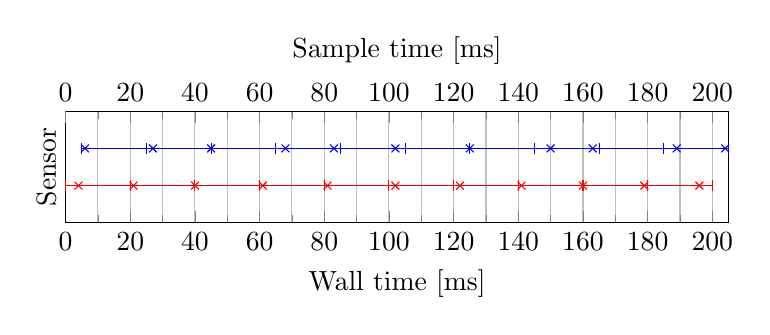
\begin{tikzpicture}
    \begin{axis}[
      height=3cm, 
      width=10cm, 
      xminorgrids=true,
      xmajorgrids=true,
      xlabel={Wall time [ms]}, 
      ylabel={Sensor},
      ytick=\empty,
      yticklabels=\empty,
      xmin=0,xmax=205,
      ymin=0,ymax=3,
      minor tick num=1,
      legend pos=south east,
      legend cell align={left}
      ]

      \addplot[color=red,mark=|] coordinates {
        (0,   1) 
        (20,  1)
        (40,  1)
        (60,  1)
        (80,  1)
        (100, 1)
        (120, 1)
        (140, 1)
        (160, 1)
        (180, 1)
        (200, 1)
      };
      \addplot[color=blue,mark=|] coordinates {
        (5,   2)
        (25,  2)
        (45,  2)
        (65,  2)
        (85,  2)
        (105, 2)
        (125, 2)
        (145, 2)
        (165, 2)
        (185, 2)
        (205, 2)
      };
    \end{axis}
    \begin{axis}[
      height=3cm, 
      width=10cm, 
      xmin=0,xmax=205,
      ymin=0,ymax=3,
      grid=none,
      ytick=\empty,
      yticklabels=\empty,
      minor tick num=1,
      axis x line*=top,
      axis y line=none,
      xlabel={Sample time [ms]}   
    ]
      \addplot[color=red,mark=x] coordinates {
        (4,   1)
        (21,  1)
        (40,  1)
        (61,  1)
        (81,  1)
        (102, 1)
        (122, 1)
        (141, 1)
        (160, 1)
        (179, 1)
        (196, 1)
      };
      \addplot[color=blue,mark=x] coordinates {
        (6,   2)
        (27,  2)
        (45,  2)
        (68,  2)
        (83,  2)
        (102, 2)
        (125, 2)
        (150, 2)
        (163, 2)
        (189, 2)
        (204, 2)
      };
    \end{axis}
  \end{tikzpicture}
  \caption{Timing errors}
  \label{plot:timing-errors}
\end{figure}

The system has to be able to cope with these misalignments and missing values: its goal is to \emph{fuse} the sensors values so that all samples appear as though they were read from a \emph{single reliable} sensor. It is also important to filter the input data to reduce the impact of noisy or faulty sensors\footnote{Accelerometers can produce noisy readings when there is no movement}; see \autoref{fig:acc}.

\fig{acc.png}{acc}{Sensor readings raw \& filtered}

The area \circled{1} in \autoref{fig:acc} shows area of no movement, but the sensor nevertheless records significant noise; \circled{2} is an example of incorrect sensor reading--humans simply cannot accelerate at \SI{5}{\meter\second^{-2}} in the \SI{20}{\milli\second} period of one sample; \circled{3} is another example of faulty sensor reading. A low-pass filter removes most of the noise, though it does not deal with possible missing values.

A good way to tackle the noise, alignment, and timing errors is to use the raw samples read from the sensors as an input to a model, and then to use the model as the source of the precise samples. \autoref{fig:sf-gaps} shows the performance of a time-series prediction algorithm applied to gaps of 15 samples--the prediction is fairly accurate in the gaps \circled{1} and \circled{2}, but fails in \circled{3}.

\fig{sf-gaps.png}{sf-gaps}{Extrapolating missing values}

\subsection{Low-power sensors}
Low-powered sensors bring additional complexity of restricted memory and computational resources, as well as restricted transfer mechanisms. A good example of such low-powered sensor is the Pebble smartwatch. The first model contains the Cortex-M3 CPU at \SI{64}{\mega\hertz} with \SI{24}{\kibi\byte} of memory (heap and code) for applications. It uses BLE for data transfers. The protocol as well as the hardware architecture places restrictions on the sample width and sampling rate. BLE protocol specifies maximum \SI{80}{\byte} per message, and minimum duration of \SI{7.5}{\milli\second} between messages; this gives a theoretical maximum of \SI{10640}{\byte\per\second}. The Pebble implementation dropped the reliable data transfer rate to only \SI{280}{\byte\per\second}. To minimise the amount of data being transferred, the system takes into account maximum reasonable acceleration a human can achieve in exercise: \SI{\pm40}{\meter\second^{-2}}, and represents that range as \SI{13}{\bit} integer. This means one sample is \SI{5}{\byte}: 3 $\times$ \SI{13}{\bit} for $x$, $y$, and $z$ axes, with \SI{1}{\bit} for padding. Along with the samples, the wearable sends its timestamp, which is a monotonously-increasing device time in milliseconds. The mobile application remembers the first seen timestamp from each sensor for each exercise session, and uses this value to properly align the samples from the sensors. The sensor data includes quantisation error: at \SI{50}{\hertz} one sample represents \SI{20}{\milli\second} of real-time, but the difference of the timestamps may not be divisible by $20$. It is sufficient to perform ``round-even'' correction of the received samples by evenly removing or duplicating the last sample in case of detected quantisation errors\footnote{Without the quantisation error correction, together with the unreliable sensors, the time error can add up to \SI{10}{\second} per hour of exercise}. 

\section{Mobile application}
Even though modern smart-watches are powerful enough to perform most of the computation, their screen sizes are a bit too small to display all the necessary information; most importantly, though, a smart-watch provides only one set of sensors. This means that exercises where the wrist where the user wears the watch does not move would not be possible to recognise. This is where the mobile application comes in: if the user places the mobile in his or her pocket, we have another sensor source. 

Crucially, all models that the mobile application needs are local to the device--the models are downloaded at application start-up (using the details embedded in the authentication JWT). The models are the nodes and transitions for the Markov chain, the neural net parameters for the set-up movement and movement classifiers. The mobile application's core functionality is packed into three components: \pcode{Predictor}, \pcode{Classifier}, and \pcode{SignalProcessor}. Perhaps counter-intuitively, the \pcode{Predictor} is the most important element of the user experience. If it makes the wrong predictions, \emph{the paper diary will be immensely more convenient}. The \pcode{Predictor} is a fairly naïve implementation of the Markov chain with \pcode{Predictor.Node} as its nodes (see \autoref{code:predictor}).

\begin{lstlisting}[caption={Predictor}, label={code:predictor}, language=swift, escapechar=|]
class Predictor {
  func predict() -> ScoredSet<Node> { ... }
  func update(taken: Node) { ... }

  enum Node {
    case exercise(label: String, 
                  duration: TimeInterval?, 
                  weight: Double?, 
                  intensity: Double?)
    case rest(duration: TimeInterval?)
  }
    
}
\end{lstlisting}

If the \pcode{Predictor} predicts exercise (with sufficient probability), it will then use the \pcode{Classifier} initialised with the set-up movement model to try to find movement that is consistent with getting ready for the exercise. Its public interface is shown in \autoref{code:classifier}.

\begin{lstlisting}[caption={Classifier}, label={code:classifier}, language=swift, escapechar=|]
class Classifier {
  
  func classify(fsd: FusedSensorData) -> 
    ScoredSet<String> {
    ...
  }
    
}
\end{lstlisting}

Before Core ML\cite{coreml}, the application included own hand-rolled forward-propagator configured with the appropriate model. It explicitly modelled the activation functions, convolution, and fully-connected layers as runtime structures. (See \autoref{code:nn}.)

\begin{lstlisting}[caption={Runtime structures for NN}, label={code:nn}, language=swift, escapechar=|]
enum ActivationFunction {
  case identity
  case sigmoid
  case tanh
  ...
}

enum LayerConfiguration {
  case fullyConnected(size: Int, weights: [Float], 
                      function: ActivationFunction)
  case convolution(...)
  ...
}

class ForwardPropagator {
  typealias Element = Float
  private let featureVectorSize: Int
  private let predictionVectorSize: Int
  private let layers: [LayerConfiguration]
  
  init(data: NSData) throws {
    ...
  }
}
\end{lstlisting}

Using the SIMD functions for the computational steps gave the application good power-efficiency compared a pure CPU-bound implementation, but larger networks brought significant memory impact (viz \autoref{code:simd}).

\begin{lstlisting}[caption={SIMD}, label={code:simd}, language=swift, escapechar=|]
extension ActivationFunction {

  func apply(inout input: [Float], 
             ofs: Int, len: Int) {
    switch self {
    case .identity: 
      |$x$|
      return
    case .sigmoid:
      |$1/(1 + e^{-x})$|
      vDSP_vneg; vvexpf; vDSP_vsadd; vvpowsf
    case .softmax:
      |$e^{x_k} / \sum_{i=1}^{len} e^{x_i}$|
      vDSP_maxv; vDSP_vsadd; vDSP_sve; vDSP_vsdiv
    ...
    }
    
}
\end{lstlisting}

With Core ML's availability, the application's code has become even more energy and memory efficient, though at the small expense of pre-compiling the newly downloaded models from the server. Finally, \autoref{code:signal-processor} shows that the interface for the signal processor--the \pcode{SignalProcessor}--is just as simple; however, the implementation again makes most of the SIMD processing capabilities in iOS.

\begin{lstlisting}[caption={Signal processor}, label={code:signal-processor}, language=swift, escapechar=|]
class SignalProcessor {
  
  func process(fsd: FusedSensorData) -> [Element] { 
    var conv = fsd.newBuffer(padded: false)
    var corr = fsd.newBuffer(padded: false)

    |Convolve the different dimensions to a single one by smoothing|
    |and adding them together|
    fsd.forEach { (dim, signal, length) in
      vDSP_vadd(&conv,   vDSP_Stride(1),
                &signal, vDSP_Stride(1),
                &conv,   vDSP_Stride(1),
                vDSP_Length(length))
    }

    |Compute autocorrelation of the padded signal with itself|
    var paddedSignal = fsd.newBuffer(padded: true)
    vDSP_conv(&paddedSignal, ..., &corr, ...)

    |Normalize the correlation values between 1 and -1|
    vDSP_vsmsa(&corr, vDSP_Stride(1), ...)

    |Count peaks; measure jitter, etc|
    return []
  }
    
  enum Element {
    case repetitions(repetitions: Int)
    case intensity(intensity: Double)
    ...
  }
}
\end{lstlisting}

Even though this code required significant effort, it meant that all processing could be kept on the device. No sensor--biometric!--data has to be sent for further processing. Even if privacy were not a concern, processing the sensor data on the server would bring unacceptable latency; it would significantly increase the application's energy impact (the radios would have to be kept on); it would also significantly increase the server-side processing bills! 

\section{Server}
Even though the mobile application can handle all the required computation for a single user, a server-side code is still required to be able to create and then improve the models that the mobile code runs. In a machine learning system, the most valuable component is the data. The first consideration is the data size: after compression, \SI{1}{\hour} of sensor data (accelerometer and gyroscope from the wrist; accelerometer and gyroscope from the waist; heart rate) and metadata (coarse and fine location, Markov chains, labels) takes up approximately \SI{2}{\mebi\byte}. This \SI{1}{\hour} represents a typical exercise session; with just 1000 users (with 50 \% training load) the system ingests \SI{1}{\gibi\byte} every day. Even though the mobile application uses lightweight touch to upload the data with the \pcode{URLSession} and \pcode{URLSessionDataTask} with the background priority, but the server still needs to handle bursts of uploads that happen when a large number of users finish their workouts: typically around 0830, and then again around 1800 during workdays, and around 1000 and 1500 during weekends. It is possible to save some of the computation and storage costs: approximately 10 \% of the users consistently mis-label their exercises\footnote{Bad number of repetitions, bad intensity, bad labels; not through malice, but by simply changing their minds. They \emph{intend to} to exercise \name{A}, but end up doing \name{B} using the same equipment or station; sometimes, they even change half-way through the exercise}; if the server side code can detect this, it can remove the \pcode{upload} claim from the JWT issued to the client application. Even without attempting to reduce the load, the good news is that for a low number of users (around 1000), AWS's \name{free usage tier} covers the required \SI{500}{\gibi\byte} storage, including the data transfer charges; the compute costs come to approximately \$60 per month. The performance requirements for the storage, model compute, and general compute resources for 1000 users form the baseline measurement; \autoref{plot:monthly-costs} shows the estimates for the costs for larger number of users. 

\begin{figure}[h]
  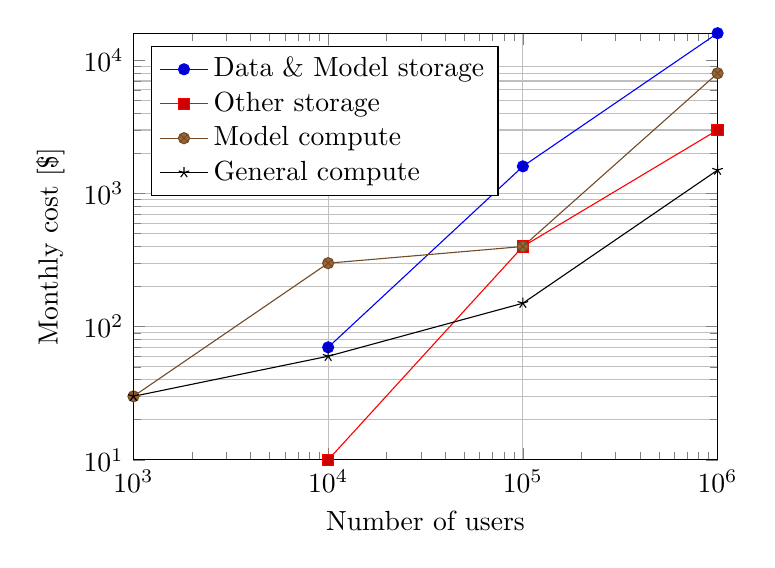
\begin{tikzpicture}
    \begin{axis}[
      height=7cm, 
      width=9cm, 
      yminorgrids=true,
      xmajorgrids=true,
      xmode=log,
      ymode=log,
      xlabel={Number of users}, 
      ylabel={Monthly cost [\$]},
      xmin=1000,xmax=1000000,
      ymin=10,ymax=16000,
      legend pos=north west,
      legend cell align={left}
      ]

      \addplot coordinates {
        (1000, 0)
        (10000, 70)
        (100000, 1600)
        (1000000, 16000)
      };
      \addlegendentry{Data \& Model storage}

      \addplot coordinates {
        (1000, 0)
        (10000, 10)
        (100000, 400)
        (1000000, 3000)
      };
      \addlegendentry{Other storage}

      \addplot coordinates {
        (1000, 30)
        (10000, 300)
        (100000, 400)
        (1000000, 8000)
      };
      \addlegendentry{Model compute}

      \addplot coordinates {
        (1000, 30)
        (10000, 60)
        (100000, 150)
        (1000000, 1500)
      };
      \addlegendentry{General compute}

    \end{axis}
  \end{tikzpicture}
  \caption{Monthly costs}
  \label{plot:monthly-costs}
\end{figure}

The costs for the \numprint{1000000} users are just an illustration: in addition to the transfer, storage, and compute resources, deployment of this scale will need additional infrastructure, monitoring; multi-region deployment for resilience will also need to be considered. Finally, the scaling requirements for the services may require some of the stateful components to be entirely re-architected using CQRS/ES architecture and reactive toolkits such as Akka\cite{akka}. Nevertheless, with a low number of users and low peak loads, the system runs on AWS using as much of the \name{free usage tier} as possible. In addition to the ALB, the server-side code uses S3 for data and model storage, DynamoDB for the profile and authorisation stores, and AWS Lambda (with Golang) for ingestion. \autoref{fig:arch} shows the main components and the relevant technologies.

\fig{arch.png}{arch}{Overall architecture}

\subsection{Ingestion \& storage}
S3, Go.

\subsection{ML} 
Hyper-parameter optimisation. Model management.

\section{Privacy}
Privacy and security of the data is extremely important. The user details that the \name{profile} service holds are ``bad enough'', but when combined with the data held in the \name{cluster} and \name{ingest} services, it must be stored and processed with the highest standards--especially with the upcoming GDPR\cite{gdpr} directive coming into force. Security and privacy extends all the way to the mobile applications and the sensors. (\cite{Fu:AuI932n8} explores viable attacks on sensors.) Naturally, the system applies encryption-at-rest to the data that the \name{profile} service holds; and the communication between the \name{profile} service and the mobile application uses transport-layer encryption. Additionally, the system does not leak the raw and stable user identity outside its infrastructure; it isolates its services in a way that programming error (\name{A2:2017}: broken authentication, \name{A5:2017}: broken access control, \name{A6:2017}: security misconfiguration, \name{A8:2017}: insecure deserialisation from the OWASP\cite{owasp} list) does not lead to \name{A3:2017}: sensitive data exposure. The system uses JWT\cite{jwt} as the authorization holder. The token holds the \pcode{cluster identifier} in the HMACSHA256-signed, base-64 encoded section, and the \pcode{user identifier} in an PKCS8-encrypted section. When the \name{authz} service issues the token it encrypts the profile-related sub-token using the \name{profile} service's public key, adds the ``public'' cluster identifier, signs the entire token and delivers it to the clients. \autoref{fig:authz} illustrates the entire flow.

\fig{authz.png}{authz}{Authorization and data access}

Initially, in \circled{1} and \circled{1$\prime$} the \name{authz} and \name{profile} service have access to a key pair; the \name{authz} service can access the public key, the \name{profile} service can access the private key. (The implementation does not naturally have access to the actual keys, it relies on a mechanism that issues a public key when it generates and securely stores a private key; it then accepts requests to decrypt a payload using the private key it holds.) The \name{authz} service then issues a token \circled{2}; the token includes encoded \& signed-only portion containing only information that cannot identify individual users, and an encrypted portion containing the user identity. The \name{ingest} \circled{3} and \pcode{model} \circled{3$\prime$} services do not have access to the private key used to encrypt the JWE token embedded in the JWT. They can use the token to authenticate access, and they use and persist the cluster identifier in their data stores. The \name{profile} \circled{5} service is able to authenticate the requests, but it can also decrypt the JWE token to obtain the user identity.

It is important to highlight that in good microservice-based architecture the services do not share data stores. Services that share a data store become tightly coupled: it is difficult for the services to have independent life-cycle, it is difficult to reason about consistency of the data across the services, and it becomes difficult to reason about authorization to access the data in the shared store.
This system avoids the sharing data stores anti-pattern; it is very explicit about how the information flows through the system. Ultimately, each service is fully responsible for its data store; each service's data store is never shared amongst other services and there are no writes that subvert the microservice's code.
A practical consequence for our system is that it is difficult to associate the session data (which contains the users' biometric data together with their location; very private information indeed) with a particular user's profile\footnote{The system does not add noise to the recorded data to further complicate the association; without the noise, it is easier--though still \emph{extremely} difficult to identify a user based on just the way he or she moves. Nevertheless, it is still impossible to tie this identification with the information held in the profile database.}. 

\section{Further work}
There is a lot of further areas of research. I think that exercise should firstly bring enjoyment and fun: this encourages further exercise, and only long-term sustainable exercise brings significant health benefits. The system collects all the information about the completed exercises (names, intensities, timings, sequence); it will then be useful to \emph{ask} the users to indicate their enjoyment after each exercise session. This can be as simple as \smiley{}, \neutranie{}, and \frownie{}; and then use the server-side processing to identify the exercises, their sequences, and intensities that the particular user (and other users in the same cluster) find enjoyable. Similarly, the concept of improvement needs further exploration: for some users, improvement means being able to lift more weight; but for users recovering from an injury, improvement means increasing their range of movement.

\printbibliography

\end{document} 